\documentclass[border=10pt]{standalone}
\usepackage{pgfplots}
\pgfplotsset{compat=1.18}
\begin{document}
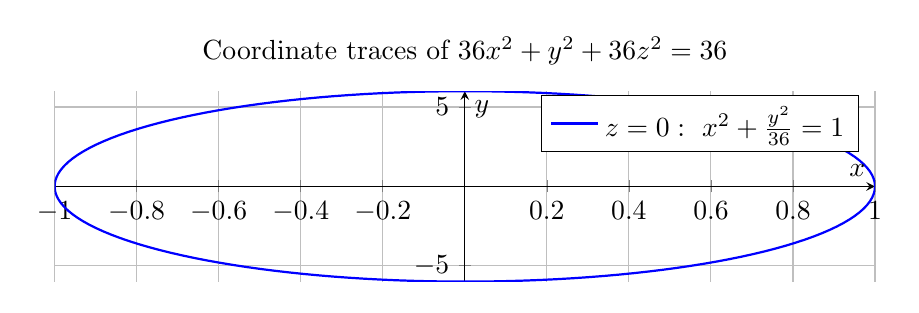
\begin{tikzpicture}
\begin{axis}[
    width=12cm,
    height=4cm,
    title={Coordinate traces of $36x^2+y^2+36z^2=36$},
    grid=major,
    axis lines=middle,
    xlabel={$x$},
    ylabel={$y$}
]
\addplot[domain=0:360, samples=160, blue, thick] ({cos(x)}, {6*sin(x)});
\addlegendentry{$z=0:\ x^2+\frac{y^2}{36}=1$}
\end{axis}
\end{tikzpicture}

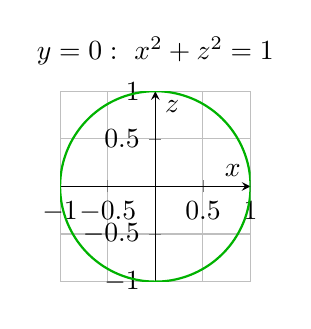
\begin{tikzpicture}
\begin{axis}[
    width=4cm,
    height=4cm,
    title={$y=0:\ x^2+z^2=1$},
    grid=major,
    axis lines=middle,
    xlabel={$x$},
    ylabel={$z$}
]
\addplot[domain=0:360, samples=160, green!70!black, thick] ({cos(x)}, {sin(x)});
\end{axis}
\end{tikzpicture}

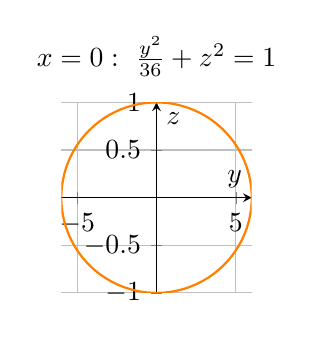
\begin{tikzpicture}
\begin{axis}[
    width=4cm,
    height=4cm,
    title={$x=0:\ \frac{y^2}{36}+z^2=1$},
    grid=major,
    axis lines=middle,
    xlabel={$y$},
    ylabel={$z$}
]
\addplot[domain=0:360, samples=160, orange, thick] ({6*sin(x)}, {cos(x)});
\end{axis}
\end{tikzpicture}
\end{document}